%% This is file `elsarticle-template-1a-num.tex',
%%
%% Copyright 2009 Elsevier Ltd
%%
%% This file is part of the 'Elsarticle Bundle'.
%% ---------------------------------------------
%%
%% It may be distributed under the conditions of the LaTeX Project Public
%% License, either version 1.2 of this license or (at your option) any
%% later version.  The latest version of this license is in
%%    http://www.latex-project.org/lppl.txt
%% and version 1.2 or later is part of all distributions of LaTeX
%% version 1999/12/01 or later.
%%
%% The list of all files belonging to the 'Elsarticle Bundle' is
%% given in the file `manifest.txt'.
%%
%% Template article for Elsevier's document class `elsarticle'
%% with numbered style bibliographic references
%%
%% $Id: elsarticle-template-1a-num.tex 151 2009-10-08 05:18:25Z rishi $
%% $URL: http://lenova.river-valley.com/svn/elsbst/trunk/elsarticle-template-1a-num.tex $
%%
\documentclass[preprint,12pt,review]{elsarticle}
\usepackage{amssymb,amsmath}
\usepackage{subfig}
\usepackage[nomarkers,nofiglist]{endfloat}
\usepackage[nodots,nocompress]{numcompress}
%Definitions
\newcommand{\bv}[1]{\mathbf{#1}} 
\newcommand{\req}[1]{#1^{*}} 

%% Use the option review to obtain double line spacing
%% \documentclass[preprint,review,12pt]{elsarticle}

%% Use the options 1p,twocolumn; 3p; 3p,twocolumn; 5p; or 5p,twocolumn
%% for a journal layout:
%% \documentclass[final,1p,times]{elsarticle}
%% \documentclass[final,1p,times,twocolumn]{elsarticle}
%% \documentclass[final,3p,times]{elsarticle}
%% \documentclass[final,3p,times,twocolumn]{elsarticle}
%% \documentclass[final,5p,times]{elsarticle}
%% \documentclass[final,5p,times,twocolumn]{elsarticle}

%% if you use PostScript figures in your article
%% use the graphics package for simple commands
%% \usepackage{graphics}
%% or use the graphicx package for more complicated commands
\usepackage{graphicx}
%% or use the epsfig package if you prefer to use the old commands
%% \usepackage{epsfig}

%% The amssymb package provides various useful mathematical symbols
\usepackage{amssymb}
%% The amsthm package provides extended theorem environments
\usepackage{amsthm}

%% The lineno packages adds line numbers. Start line numbering with
%% \begin{linenumbers}, end it with \end{linenumbers}. Or switch it on
%% for the whole article with \linenumbers after \end{frontmatter}.
%\usepackage{lineno}

%% natbib.sty is loaded by default. However, natbib options can be
%% provided with \biboptions{...} command. Following options are
%% valid:

%%   round  -  round parentheses are used (default)
%%   square -  square brackets are used   [option]
%%   curly  -  curly braces are used      {option}
%%   angle  -  angle brackets are used    <option>
%%   semicolon  -  multiple citations separated by semi-colon
%%   colon  - same as semicolon, an earlier confusion
%%   comma  -  separated by comma
%%   numbers-  selects numerical citations
%%   super  -  numerical citations as superscripts
%%   sort   -  sorts multiple citations according to order in ref. list
%%   sort&compress   -  like sort, but also compresses numerical citations
%%   compress - compresses without sorting
%%
%% \biboptions{comma,round}

% \biboptions{}


%\journal{Journal Title}

\begin{document}

\begin{frontmatter}

%% Title, authors and addresses

%% use the tnoteref command within \title for footnotes;
%% use the tnotetext command for the associated footnote;
%% use the fnref command within \author or \address for footnotes;
%% use the fntext command for the associated footnote;
%% use the corref command within \author for corresponding author footnotes;
%% use the cortext command for the associated footnote;
%% use the ead command for the email address,
%% and the form \ead[url] for the home page:
%%
%% \title{Title\tnoteref{label1}}
%% \tnotetext[label1]{}
%% \author{Name\corref{cor1}\fnref{label2}}
%% \ead{email address}
%% \ead[url]{home page}
%% \fntext[label2]{}
%% \cortext[cor1]{}
%% \address{Address\fnref{label3}}
%% \fntext[label3]{}

\title{Eulerian-Lagrangian Simulation of a Turbulent Evaporating Spray using RANS Modeling}

%% use optional labels to link authors explicitly to addresses:
%% \author[label1,label2]{<author name>}
%% \address[label1]{<address>}
%% \address[label2]{<address>}

\author[]{\textbf{Rodrigo B. Piccinini}\\ \textbf{Marcelo J.S. de Lemos}$^{*}$}
\address{Departamento de Energia - IEME \\
Instituto Tecnol\'{o}gico de Aeron\'{a}utica - ITA\\
12228-900 - S\~{a}o Jos\'{e} dos Campos - SP, Brazil\\
$^{*}$\textit{\textbf{Corresponding author} E-mail: \underline{delemos@ita.br}}}


\begin{abstract}
RANS simulation is applied to a turbulent and evaporating spray of acetone in an air co-flow stream. The air is a continuous phase in an Eulerian description and the liquid is a dispersed phase of point-particles in a Lagragian description. An  approximation of zero Mach number was applied to the governing equations of the continuous phase. Turbulence was modeled using k-epsilon model. Submodels were used for heat and mass inter-phase transfers and Nusselt and Sherwood numbers are given by empirical correlations for convective droplet heating and evaporation. The spray interaction with turbulence is only accounted for in droplet motion using the random walk procedure. The numerical results were compared to measurements and a reasonable prediction was found for droplet and gas velocities and liquid evaporation, although underestimated.
\end{abstract}

\begin{keyword}
%% keywords here, in the form: keyword \sep keyword

%% MSC codes here, in the form: \MSC code \sep code
%% or \MSC[2008] code \sep code (2000 is the default)
spray \sep round jet \sep low Mach number \sep lagrangian \sep point-particle method
\end{keyword}

\end{frontmatter}

\begin{tabular}{ll}
\textbf{Nomenclature:} & \\
$C_D$ & doplet drag coefficient \\
$c_p$ & specific heat at constant pressure [$J/kg/K$] \\
$D$ & droplet diameter [$m$]\\
$\tilde{f}$ & favre-average of function $f$\\
$f''$ & deviation of favre-averaged function $\tilde{f}$\\
$\bar{f}$ & time-average of function $f$\\
$f'$ & deviation of time-averaged function $\bar{f}$\\
$\bv{g}$ & vector field of gravity force [$m/s^2$]\\
$\dot{m}_d$ & mass flow rate of liquid injection [$kg/s$]\\
$\dot{m}_{g}$ & gas mass rate [$kg/s$]\\
$\dot{m}_{vapor}$ & acetone vapor mass rate [$kg/s$]\\
$h_d$ & droplet enthalpy [$J/kg$]\\
$h_s$ & gas sensible enthalpy [$J/kg$]\\
$k$ & turbulent kinetic energy [$J/kg$]\\
$\hat{k}$ & jet dimensionless $k$: $\hat{k}=k/(\tilde{U}_{x,0}-\tilde{U}_{cl})^2$ \\
$L_v$ & latent heat of vaporization [$J/kg$]\\
$m_d$ & droplet mass [$kg$]\\
$M$ & Mach number \\
$p_{0}$ & thermodynamic pressure [$Pa$]\\
$p_{2}$ & dynamic pressure [$Pa$]\\
$p$ & pressure [$Pa$]\\
$Pr$ & Prandtl number \\
\end{tabular}

\vspace{25pt}

\begin{tabular}{ll}
$Re_d$ & droplet Reynolds number, $Re=(\rho |\bv{U}|_{slip} D) /\mu$ \\
$S_{hs}$ & spray enthalpy source term [$J/m^3/s$]\\
$S_{m}$ & spray mass source term [$kg/m^3/s$]\\
$S_{mom}$ & spray momentum source term [$kg/m^3/s$]\\
$S_{Y_k}$ & spray source term of species k [$kg/m^3/s$]\\
$Sc$ & Schmidt number \\
$Sh$ & Sherwood number \\
$T_d$ & droplet temperature [$K$]\\
$T$ & gas temperature [$K$]\\
$t$ & time [$s$]\\
$\bv{U}$ & gas velocity vector [$m/s$]\\
$\bv{U}_d$ & droplet velocity vector [$m/s$]\\
$\bv{U}_{slip}$ & droplet velocity relative to the gas: $\bv{U}_{slip}=\bv{U}_d -\bv{U}$  [$m/s$]\\
$\tilde{U}_{x,0}$ & jet centerline velocity \\
$\tilde{U}_{x,cf}$ & co-flow velocity \\
$\hat{U}$ & dimensionless jet velocity, $\hat{U} = (\tilde{U}_x-\tilde{U}_{x,cf})/(\tilde{U}_{x0}-\tilde{U}_{x,cf})$ \\
$y_{1/2}(x)$ & jet half-radius, the radial coordinate for which $\tilde{U}_x (y=y_{1/2}) = 1/2\tilde{U}_{x,0}$\\
$\hat{y}(x,y)$ & dimensionless radial coordinate: $\hat{y}(x,y)=y/y_{1/2}$ \\
$x$ & axial coordinate [$m$]\\
$\bv{x}$ & position vector [$m$] \\
$y$ & radial coordinate [$m$]\\
$Y_k$ & mass fraction of species k\\
$W_k$ & molecular weight of species k [$kg/mol$]\\
\end{tabular}

\vspace{25pt}

\begin{tabular}{ll}
\textbf{Greek Characters:} & \\
$\alpha$ & thermal diffusivity [$m^2/s$]\\
$\gamma$ & ratio of constant pressure and constant volume specific heats \\
$\epsilon$ & dissipation rate of turbulent kinetic energy [$J/kg/s$]\\
$\kappa$ & thermal conductivity [$W/m/K$]\\
$\mu$ & gas dynamic viscosity [$Pa.s$]\\
$\nu$ & gas kinematic viscosity [$m^2 /s$]\\
$\nu_T$ &  turbulent viscosity [$m^2 /s$] \\
$\hat{\nu}_T$ &  jet dimensionless turbulent viscosity: $\hat{\nu}_T = \mu/(\bar{\rho}\tilde{U}_{x,0} y_{1/2})$\\
$\rho$ & gas density [$kg/m^3$]\\
$\rho_d$ & droplet density [$kg/m^3$]\\
$\bv{\tau}$ & viscous stress tensor [$Pa$]\\
$\tau_e$ & droplet evaporation relaxation time [$s$]\\
$\tau_h$ & droplet heating relaxation time [$s$]\\
$\tau_u$ & droplet momentum relaxation time [$s$] \\
$\phi_{v,l}$ & liquid volume fraction
\end{tabular}

\vspace{25pt}

\begin{tabular}{ll}
\textbf{Special Characters:} & \\
cdf & cumulative density function\\
pdf & probability densitiy function\\
pmf & probability mass function\\
SMD & Sauter mean diameter \\
$\mathcal{D}_k$ & binary diffusion coefficient of species k [$m^2/s$]
\end{tabular}


%%
%% Start line numbering here if you want
%%
% \linenumbers

%% main text
\section{Introduction}
\label{intro}
A spray jet is a particular case of a dispersed multiphase flow originated by the instabilization of a liquid jet emerging in a gaseous atmosphere.  The spray is composed by the continuous gaseous phase and the dispersed phase of liquid droplets.
Depending on the liquid volumetric fraction, the spray may be classified as dense ($\phi_l > 10^{-3}$) or dilute ($\phi_l \le 10^{-3}$). The dilute sprays are commonly modeled using the so called two-way coupling, where interaction between gas and liquid droplets is modeled, but interaction among droplets is neglected.

RANS modeling has been extensively used to spray jets simulations, see \citet{baumgarten2006mixture}, and, more recently, large-eddy (LES) and direct simulations (DNS) have also been applied. Independently on the turbulence modeling, droplet heating and evaporation are often similarly modeled with empirical correlations for Nusselt and Sherwood numbers, such as those of Ranz and Marshall's \citet{ranzmarshall}. This indicates that much of the improvement obtained in LES simulations in the prediction of droplet velocity and evaporation rate, e.g. \citet{bini} and \citet{moin},  was due to the best modeling of turbulent motion and the allowance of gas properties such as temperature ($T$) and species mass fractions ($Y_k$) to deviate from mean values. It certainly provides a more accurate description of droplet environment in a turbulent spray jet. Actually, \citet{bini} has also shown that subgrid modeling of Sherwood number in LES further improved predictions of droplet evaporation.

This scenario suggests the possibility of improving RANS simulations with stochastic submodeling of not only droplet dispersion, but of heat and mass transfers as well. Also, the proposition of RANS submodels would certainly benefit from the results coming from LES and DNS.

This paper presents results of applying RANS modeling to the experiment developed by \citet{chen}. It has found overestimation of jet spread rate using the usual coefficients of k-epsilon model and underprediction of droplet velocity and evaporation rate, specially after the the jet core. It suggests that future modification of turbulence model coefficients and stochastic submodels for heat and mass transfers could improve predictions.

\section{Governing Equations}
\label{equations}


\subsection{Continuous Phase}\label{continuous_phase}
The equations for the continuous gaseous phase were derived from the fully compressible formulation, \citet{poinsot2005theoretical}, with additional spray source terms ($S_m$, $S_Y$, $S_{mom}$ and $S_{hs}$). It was applied the low Mach number approximation, see \citet{majda}, and performed the Reynolds and Favre averages for turbulence modeling.

The low Mach number approximation expands all variables in power series of $\xi=\sqrt{\gamma}M^2$ and only collects the equations of zeroth order in $\xi$. This procedure splits pressure in two parcels,
\begin{equation}
p = p_{0}(t) + p_{2}(\bv{x},t)\xi^2 + O\left( \xi^3 \right) \, .
\end{equation}
$p_0$ is called the thermodynamic pressure, it is shown to be function of time only and it is present in the state and energy equations; $p_1$ is not present in the equations for zeroth order terms and $p_2$ is the dynamic pressure, whose gradient is present in the momentum equation.

The continuity equation reads:
\begin{equation}\label{av: mass}
  \frac{\partial \bar{\rho}}{\partial t} + \nabla \cdot \left( \bar{\rho}
\tilde{\bv{U}} \right) =  \bar{S}_m \, .
\end{equation}

The acetone ($Y_{ac}$) conservation equation for binary diffusion and unitary Schmidt number reads:
\begin{equation}\label{av: species}
 \frac{\partial \bar{\rho} \tilde{Y}_{ac} }{\partial t} + \nabla
\cdot\left(\bar{\rho} \tilde{\bv{U}} \tilde{Y}_{ac} \right) = \nabla \cdot \left[ \bar{\rho} \left( \nu + \nu_T \right)
\nabla \tilde{Y}_{ac} \right] +\bar{S}_{Yac} \, ,
\end{equation}
air is treated as an inert species with
\begin{equation}
\tilde{Y}_{air} = 1- \tilde{Y}_{ac} \, .
\end{equation}

The momentum equation reads:
\begin{equation}\label{av: momentum}
 \frac{\partial \bar{\rho} \tilde{\bv{U}} }{\partial t} + \nabla \cdot \left(
\bar{\rho} \tilde{\bv{U}} \tilde{\bv{U}} \right) = -\nabla \bar{p}_2 +  
 \nabla \cdot\overline{\bv{\tau}} +\bar{\rho}\bv{g}+\bar{\bv{S}}_{mom}  \, .
\end{equation}
where $\bv{\tau}$ is the viscous stress tensor with effective viscosity $\mu_{eff}=\mu+\mu_T$. 

The energy equation is written in terms of sensible enthalpy with unitary turbulent Prandtl number:
\begin{equation}\label{av: enthalpy}
\frac{\partial \bar{\rho} \tilde{h}_{s}}{\partial t} + \nabla \cdot
\left(\bar{\rho} \tilde{\bv{U}} \tilde{h}_{s} \right) = \nabla \cdot \bar{\bv{J}}_s + \bar{S}_{hs}\, ,
\end{equation} where 
\begin{equation}
\bar{\bv{J}}_s =  \bar{\rho} \left( \alpha + \nu_T\right) \nabla \tilde{h}_s \, .
\end{equation}
The pressure work ($Dp/Dt$ ) and species thermal diffusion were neglected.

State Equation is:
\begin{equation}
  \bar{p}_0 W = R \bar{\rho} \tilde{T} 
\end{equation}

The k-epsilon equations are those presented in \citet{nordin} with $\dot{W}^{s}= 0$, that is, no sink of turbulent kinetic energy was defined here due to the work done by the eddies on the droplets. The model has six parameters whose values are shown in Table \ref{table: kepscoeff}.

\section{Dispersed Phase}\label{dispersed_phase}

The dispersed phase is written in a Lagrangian reference frame. The droplet equations are:
\begin{align}\label{eq: drop_dudt}
\text{Momentum:}&\quad \frac{d\bv{U}_d}{dt} = -\frac{ \bv{U}_{slip}}{\tau_{u}} + \bv{g}  \\
\label{eq: dropmass}
\text{Mass:}&\quad \frac{dm_d}{dt}=-\frac{m_d}{\tau_e} \, , \\
\text{Energy:}&\quad \frac{dT_d}{dt}= \frac{T-T_d}{\tau_h} f - \frac{1}{c_{p,d}} \frac{L_v\left( T_d\right) }{\tau_e}
\end{align}

In the momentum equation, $\tau_u$ is the momentum relaxation time:
\begin{equation}
 \tau_u = \frac{8 m_d}{\pi \rho C_D D^2 | \bv{U}_{slip}|}=\frac{4}{3}
\frac{\rho_d D}{\rho C_D | \bv{U}_{slip}|} \, .
\end{equation}
The drag coefficient ($C_D$) is computed using the expression in \citet{nordin}.
The droplet slip velocity is:
\begin{equation}\label{eq: Urel}
 \bv{U}_{slip} = \bv{U_d} - \tilde{\bv{U}}-\bv{U}'' \, ,
\end{equation}
where $\tilde{\bv{U}}$ is the Favre-averaged gas velocity computed in Equation \eqref{av: momentum}. The fluctuation of gas velocity ($\bv{U}''$) is determined using the random walk procedure of \citet{rourke}. For the k-epsilon model, a characteristic velocity may be defined as:
\begin{equation}
 <U''>= \sqrt{\frac{2}{3} k} \, .
\end{equation}
The magnitude of the velocity fluctuation ($\bv{U}''$) is then sampled from a Gaussian distribution with a variance equal to $<U''>$ and zero mean. Finally, the direction of $\bv{U}''$  is randomly chosen.

The sampling is performed once the time passed from the last sampling is greater than the characteristic time $\tau_{turb}$: the minimum between the eddy lifetime and the time taken to the droplet to cross it, given by the ratio of a turbulent length scale ($l_t = C_{\mu}^{3/4} k^{3/2} / \epsilon $) and the magnitude of the droplet slip velocity:
\begin{equation}
 \tau_{turb} = min \left[ \frac{k}{\epsilon} , \frac{k^{3/2}}{\epsilon} \frac{C_{\mu}^{3/4}}{|\bv{U}_{slip}|}\right] \, .
\end{equation}

The characteristic time scales for heating ($\tau_h$) and evaporation ($\tau_e$) are:
\begin{equation}
 \tau_h=\frac{m_d c_{l,d}}{\pi D \kappa Nu} \, , \quad  \tau_e = \frac{m_d}{\pi D \mathcal{D} Sh \rho_v ln\left(\frac{1-Y_{v,\infty}}{1-Y_{v,s}} \right)} \, .
\end{equation}
The $f$ factor in the energy equation corrects for the heat not transfered to the droplet, but to the surrounding vapor:
\begin{equation}
f =  \frac{z}{e^z-1} \,  \quad \text{and} \quad z= - \frac{c_{p,f} \dot{m_f} B}{ \pi D^2 h_c} \, .
\end{equation}

The Nusselt and Sherwood numbers are computed from the empirical correlations of \citet{ranzmarshall}:
\begin{equation}\label{nueq}
 Nu= 2.0 +0.6 Re^{1/2} Pr^{1/3} \, ,
\end{equation}
\begin{equation}\label{sheq}
 Sh = 2.0 +0.6 Re^{1/2} Sc^{1/3} \, .
\end{equation}
They account for the extra heat and mass transfer due to gas motion around the droplet. All gas properties in Equations \eqref{nueq} and \eqref{sheq} are computed using the film temperature, see \citet{naca}.

The vapor mass fraction in the droplet surrounding ($Y_{v,s}$) is obtained assuming liquid-vapor equilibrium and using Raoult's law:
\begin{equation}
Y_{v,s} = \frac{p_v \left(T_d\right)}{p}\frac{W_v}{W} \, ,
\end{equation}
$p_v \left(T_d\right)$ is the equilibrium vapor pressure at droplet temperature $T_d$.

\section{The Experiment Configuration}
\label{experiment}
\citet{chen} performed at Sydney University a detailed experimental investigation of a turbulent evaporating jet of acetone. Droplet diameter, droplet velocity, droplet number density and liquid volumetric flux were measured using a two-component phase Doppler interferometry (PDI) and acetone vapor mass flux was measured using planar laser-induced fluorescence (PLIF).

The experiment consists of a spray nozzle centered on the exit plane of a wind tunnel with 150mm by 150mm that supplies a co-flowing air stream, see Figure \ref{spray_jet}. 
Inside the nozzle, a pressurized liquid jet is surrounded by a carrier air flow until the nozzle exit. The co-flow has a low turbulence intensity of less than $2\%$, so that the effect on the spray jet turbulence is negligible. The main benefit of this setup is the avoidance of flow recirculation near the nozzle exit, simplifying the boundary conditions for a numerical simulation.

Table \ref{table: exp} summarizes the basic characteristics of the experiment. The droplet velocities in the nozzle exit were measured and the droplet and gas temperatures were calculated from thermal equilibrium assumption. The statistical distribution of droplet diameters in the nozzle was not provided by the experiment and only the Sauter mean diameter (SMD) is known.  A lognormal distribution was then specified with expected value and standard deviation being, respectively, $E = 10\ \mu m$ and $SD=5.5\ \mu m$.

\section{Aspects of the Numerical Solution}
The numerical solution of the equations in Section \ref{equations} was obtained using finite volume method with the OpenFOAM code, more specifically the dieselFOAM solver and dieselSpray library. Minor modifications were made in order to solve for the low Mach number equations and to adapt boundary conditions to the experiment.

\subsection{Domain Discretization (The Numerical Grid)}

Two axisymmetric (2D) orthogonal mesh grids were built: a fine and a coarse grid. OpenFOAM uses the collocated grid arrangement. The fine grid was composed of $14,800$ cells ($74$ cells in the radial direction and $200$ in the axial direction) and the coarse grid was composed of $5,460$ cells ($42$ in the radial direction and $130$ in the axial direction).

Solutions for both grids were obtained for a pure gas flow. In despite of some differences, the coarse grid solution was considered enough accurate and it was used for the results presented in this paper.

Droplets were injected in the domain at a rate of $5 \times 10^5\ droplets/s$.

\subsection{Equation Discretization}

The general transport equation for a scalar intensive property $\phi$ is:
\begin{equation}
 \underbrace{\frac{\partial \rho \phi}{\partial t}}_{\text{temporal derivative}} + \underbrace{\nabla \cdot \left(\rho \bv{U} \phi \right)}_{\text{advection}} - \underbrace{\nabla \cdot \left( \rho \Gamma \nabla \phi \right)}_{\text{diffusion}} = \underbrace{S\left(\phi\right)}_{\text{source}}
\end{equation}

The discretization of each term used the following schemes:
\begin{itemize}
 \item Temporal derivative: Euler implicit method;
 \item Advection term: Gauss theorem is applied to transform the divergence in surface integrals and the upwind scheme is used to interpolate values from cell center to cell faces;
 \item Diffusion term: Gauss theorem for the divergent with linear interpolation for the diffusion coefficient from cell center to cell faces. Central difference is used for the gradient;
 \item Sources: all sprays sources are explicitly handled. The spray is evolved from time step "n" to "n+1" using the gas phase properties at time step "n", and all source terms are computed. The gas is then evolved to time step "n+1".
\end{itemize}

After discretization, the resulting algebraic equations were solved in segregated linear systems using conjugate gradient algorithms.
The pressure-velocity coupling is solved using the PISO algorithm, see \citet{issa}. In the low Mach number formulation, the convective-diffusive pressure equation for compressible flows becomes a Poisson equation as it is for incompressible flows.

\section{Results}

\subsection{Gas and Droplet Velocities and Droplet Dispersion}

An empirical observation of a gas turbulent round jet is that the profiles of $\hat{U}$, $\hat{k}$ and $\hat{\nu}_T$ as function of $\hat{y}$ becomes self-similar (i.e. independent of the axial coordinate) from some distance to the nozzle exit.
Furthermore, there is a linear relation between the half-radius ($y_{1/2}$) and the axial coordinate, that is, the jet sprad rate is constant:
\begin{equation}
S = \frac{d y_{1/2} (x)}{dx} \, .
\end{equation}

\citet{chen} has experimentally shown that self-similarity also occurred for $\hat{U}$ in the presence of the spray jet for $x/D \ge 10$. For arriving at this conclusion, it assumed the velocity measured for the smaller droplets ($D<3\mu m$) as being the gas velocity. 

The group of Figures \ref{fig: selfsimilar_profile} shows the same investigation for the gas velocity field obtained in the numerical simulation. The Figure \ref{ssA} shows the profiles of $\hat{U}$ for several axial coordinates. Differently than the experiment, the self-similarity only occurs for $x/D \ge 15$ (and not for $x/D \ge 10$). This suggests that the transition from the jet developing region to the turbulent region is retarded in the simulation.

Figures \ref{ssB} and \ref{ssC} show that the evolution to self-similar profiles is slower for the turbulent quantities $\hat{k}$ and $\hat{\nu}_T$ and one may not say that the self-similarity was achieved inside the domain. \citet{chen} has shown that for $x/D \le 25$ it was also not achieved in the experiment for the root mean square of the axial velocity fluctuation ($<U''_x>$). 

One observation concerning the turbulent viscosity ($\hat{\nu}_T$) is that the centerline value seems to evolve to a value of $\hat{\nu}_T = 0.047$, higher than values found in the literature for the turbulent round jet. \citet{pope2000turbulent} reports a self-similar turbulent viscosity at centerline of $\hat{\nu}_T = 0.029$.

The jet spread rate measures the spread of the axial velocity in the radial direction. A value about $S=0.095$ is found on the literature for the pure gas flow \citet{pope2000turbulent}, and it is independent of Reynolds number. For the spray jet, however, \citet{chen} has reported $S=0.0665$. In the simulation it was found a higher value of $S=0.071$, a difference of $23\%$. 

The Figure \ref{fig: ssS} shows the indeed different half-radius values found in the simulation and the experiment for the same axial coordinates and Figure \ref{fig: ssP} compares the self-similar profiles of $\hat{U}_x$ from the simulation and the experiment.

The overestimation of the round jet spread rate with the default coefficients of k-epsilon model has been reported previously by different authors. \citet{luppes} has discussed four alternatives to the correction. The modifications consist not only in changing the model coefficients, but also in tunning of boundary conditions. 

\subsection{Gas and Droplet Velocities and Droplet Dispersion}

\citet{chen} has presented velocity measurements for droplets of four diameter classes in the spray jet: $D< 5\mu m$, $10\mu m <D<20\mu m$, $20 \mu m < D < 30 \mu m$ and $30 \mu m < D < 40 \mu m$. The importance of separating the data in droplet size classes is that the drag force is dependent on its size. 

Figure \ref{fig: Ux_gas} shows in red squares the measured radial profiles of the mean axial velocity for the gas phase ($\tilde{U}_x$) in the axial coordinates of: $x/D=5$, $10$, $15$, $20$ and $25$. The radial profile obtained in the simulation is also shown in a solid black line. It is evident that the underprediction of the gas velocity in the simulation becomes higher in the downstream direction. In the axial coordinate of $x/D=25$, the centerline value in the simulation is about $20\%$ below the experimental value. In fact, \citet{luppes} has reported an error of the same percentual magnitude using the k-epsilon model with the default coefficients. 

\citet{chen} has also reported the root mean square of the axial and the radial velocities, respectively $<U''_x>$ and $<U''_y>$. Again, the values for the smaller droplets ($D< 5\ \mu m$) are being used to represent the gas velocity. The same quantities are not provided in the simulation for direct comparison. The turbulence model only solves for the turbulent kinetic energy and its dissipation rate. A characteristic velocity, however, may be defined as $<U''>=\sqrt{2/3 k}$. This quantity is shown in Figure \ref{fig: UUx} with $<U''_x>$ and $<U''_y>$. Again, it is shown radial profiles for different axial coordinates.

Three observations are readily made:  
\begin{itemize}
  \item The radial profile of $<U''_x>$ is similar to that of $<U''_y>$;
  \item The characteristic velocity defined for the k-epsilon model ($<U''>$) agrees well with $<U''_x>$ and $<U''_y>$;
 \item $<U''>$ declines faster than $<U''_x>$ and $<U''_y>$ as the axial coordinate increases.
\end{itemize}

The first observation indicates that the turbulent jet differs from the self-similar profiles found in the literature \citet{pope2000turbulent}, where $<U''_x>$ is about twice as big as $<U''_y>$ in the centerline. It remains the question whether this occurs because the jet is not fully developed or because of some spray influence.

The second observation suggests that the k-epsilon model is appropriate to describe the round jet turbulence, providing an appropriate characteristic velocity. The third observation, however, indicates that the turbulent dissipation is overpredicted.

Returning to the mentioned influence of the discrepancies in the mean axial velocity of the gas phase on the droplet velocities, the lower velocity of the gas increases the droplet slip velocity and causes a larger drag to be felt by them. The obvious conclusion is that the same discrepancy in the gas velocity will be observed in the comparison of experimental and numerical values for the droplet velocities.

Figure \ref{fig: Ux} shows in red squares the radial velocity profile measured  by \citet{chen} for droplets in the class of $10\mu m <D<20\mu m$ in the axial coordinates of: $x/D=5$, $10$, $15$, $20$ and $25$.  For each radial position, the velocity value is the ensemble average of the droplets crossing the laser PDI beams. The droplet velocity obtained in the simulation is also shown as black scattered points representing each of them a different droplet in the computation, no averaging was performed.

It is observed that the computed droplet velocity also becomes systematically lower than the measurements in the downstream direction.

\subsection{Liquid and Vapor Mass Fluxes}

The correct prediction of droplet evaporation is, together with the velocity, of high importance for the applications of the spray simulation. The reasonably low discrepancies found for droplet velocity in Figure \ref{fig: Ux} already indicates that the evaporation model performed well. This is due to the fact that an incorrect modeling of evaporation would lead to an erroneous droplet diameter, further affecting the velocity prediction.

Figure \ref{fig: droplet_flux} shows the numerical and the experimental liquid mass flow rate for different axial coordinates. The computed values are in good agreement with the measurements for $x/D \le 10$. Further downstream, the simulation overpredicts the liquid flow rate. Clearly, this means that droplet evaporation is lower than it should be. In fact, in Figure \ref{fig: vapor_flux}, it is made the comparison of experimental and numerical radial profiles of vapor mass fluxes and the trend is exactly the same: as the axial coordinate increases, less vapor (hence more liquid) is present in the simulation than it is in the experiment.

The underestimation of evaporation rate has also been noticed in a large-eddy simulation performed by \citet{bini}, where it was discussed the effect of a subgrid model to the evaporation. It is said that the lack of a subgrid model affects evaporation mainly in the jet core. In fact, the evaporation model presented in Section \ref{dispersed_phase} only dealt with mean flow properties and transfer coefficients, and the temperature and mass fraction oscillations, ($T''$) and ($Y''_{ac}$), were not taken into account.

Surely, for a large-eddy simulation, the lack of a subgrid model is less severe than it is in RANS modeling, since at least the non-filtered oscillations are present. 

It must also be pointed that uncertainties in the gas mean velocity also affect the prediction of droplet heating and evaporation because of the different slip velocity. The correct attempt to improve accuracy of the present computation would be to adjust the turbulence model to first correct the gas mean velocity and see the new evaporation rates. Next, a stochastic subgrid model for the heat and mass transfer coefficients could be studied.

The last studied property of the spray is the droplet Sauter mean diameter (SMD). Figure \ref{fig: SMDprofile} shows the numerical and experimental radial profiles of SMD.

The computed Sauter mean diameter shows a good agreement with measurements, in despite of the uncertainty about the droplet size distribution in the boundary conditions and the higher liquid flow rates in Figure \ref{fig: droplet_flux}. This may also be a consequence of the low variance in droplet diameter in the nozzle injection.

This agreement also confirms that the velocity discrepancy is caused by the anomalous jet spread rate. As discussed previously, if diameters were also in disagreement, the predicted drag force on the droplets would be further incorrect.

\section{Conclusions}

The velocity of both the gas and the liquid phase were underpredicted due to the high turbulent viscosity of the turbulence model. It is suggested in the literature that this discrepancies for a round jet might be diminished by changing the model coefficients and reducing the turbulent length scale in the jet inlet boundary condition.

The evaporation rate was underpredicted after the jet developing region. Turbulence effects on Nusselt and Sherwood numbers were not modeled and this is belivied to decrease evaporation, specially in the jet core, as reported by \citet{bini}.

Disagreements in the prediction of gas velocity may also have contributed to differences in the evaporation rate. The error in liquid mass flow rate at some axial location was about $20\%$.

The shape of the radial profile of vapor mass flux was well predicted. The same can be said to the SMD radial profiles.

Future work could explore improvements in the round jet turbulence modeling and new heating and evaporation models for RANS simulations accounting for fluctuations of flow properties.


%% The Appendices part is started with the command \appendix;
%% appendix sections are then done as normal sections
%% \appendix

%% \section{}
%% \label{}

%% References
%%
%% Following citation commands can be used in the body text:
%% Usage of \cite is as follows:
%%   \citet{key}          ==>>  [#]
%%   \cite[chap. 2]{key} ==>>  [#, chap. 2]
%%   \citet{key}         ==>>  Author [#]

%% References with bibTeX database:

\bibliographystyle{model1c-num-names}
\bibliography{../thesis/references.bib}
\nocite{*}
%% Authors are advised to submit their bibtex database files. They are
%% requested to list a bibtex style file in the manuscript if they do
%% not want to use model1a-num-names.bst.

%% References without bibTeX database:

% \begin{thebibliography}{00}

%% \bibitem must have the following form:
%%   \bibitem{key}...
%%

% \bibitem{}

% \end{thebibliography}

\newpage
\listoffigures

\newpage

\begin{table}
\centering
 \begin{tabular}{lc}
\hline
Experiment  Data & \\ \hline
Liquid Phase & Acetone \\
Liquid Flow rate at nozzle exit $(g/min)$  &  $7.0$ \\
Carrier air flow rate $(g/min)$ & $135$ \\
Vapor flux at nozzle exit $(g/min)$ & $5.0$ \\
SMD at nozzle exit $(\mu m)$ & $13.7$ \\
Gas temperature at nozzle exit $(K)$ & $280$ \\ 
Gas jet Reynolds Number $(Re=4 \dot{m}_g/\pi D_{nozzle} \mu_g)$ & $16,300$ \\
\hline
 \end{tabular}
\caption{Basic information about the experiment of \citet{chen}.}
\label{table: exp}
\end{table} 

\begin{table}
\centering
 \begin{tabular}{cc}
  \hline
  $C_{\mu}$ & $0.09$ \\
  $C_{\epsilon 1}$ & $1.44$ \\
  $C_{\epsilon 2}$ & $1.92$ \\
  $C_{\epsilon 3}$ & $-0.33$ \\
  $\sigma_k$ & $1$ \\
  $\sigma_{\epsilon}$ & $1.3$ \\ \hline
 \end{tabular}
\caption{k-epsilon model constants.}
\label{table: kepscoeff}
\end{table} 

\begin{figure}
 \centering
 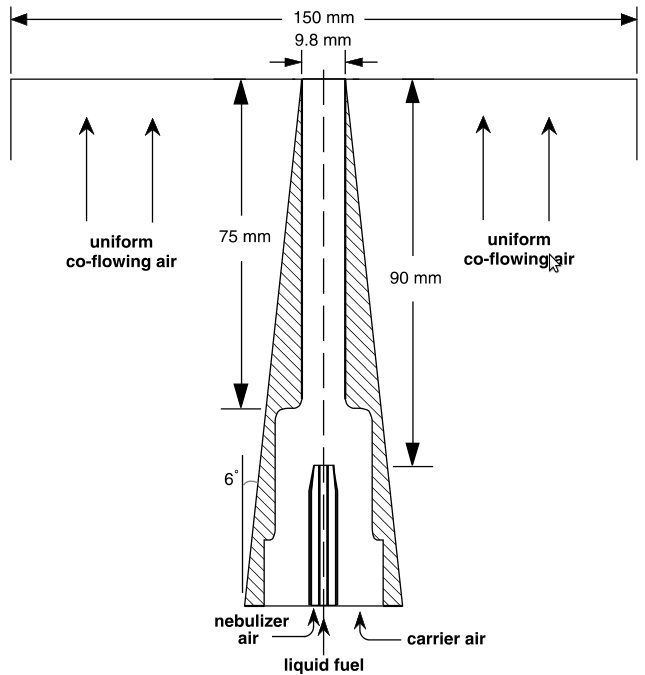
\includegraphics[width=0.75\textwidth]{../thesis/figuras/chap3/setup.png}
 % setup.png: 645x675 pixel, 72dpi, 22.75x23.81 cm, bb=
 \caption{Configuration of the spray jet nozzle of \citet{chen}.}
 \label{spray_jet}
\end{figure}


\begin{figure}[!htb]
 \centering
\begin{tabular}{cc}
 \subfloat[]{\label{ssA}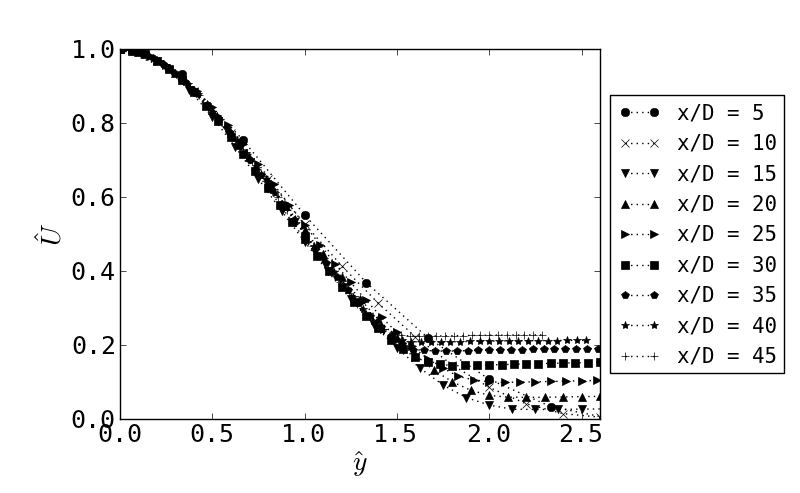
\includegraphics[width=0.5\textwidth]{../thesis/figuras/chap5/selfsimilar/selfsimilar_U.png}} &
 \subfloat[]{\label{ssB}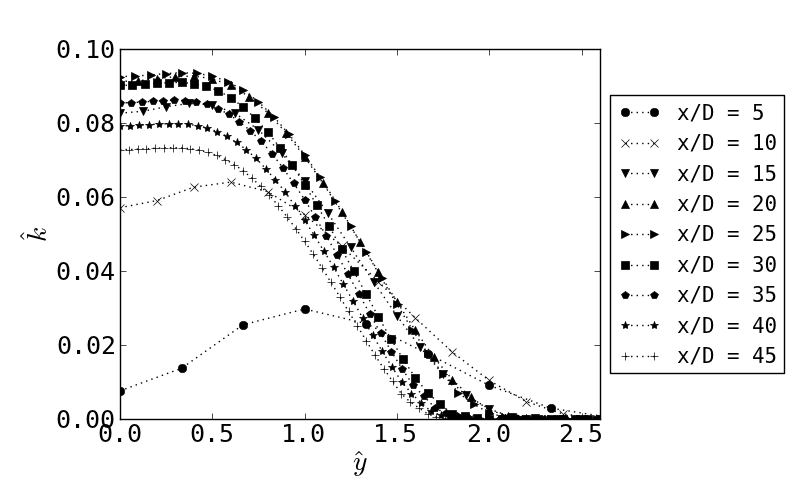
\includegraphics[width=0.5\textwidth]{../thesis/figuras/chap5/selfsimilar/selfsimilar_k.png}} \\
 \subfloat[]{\label{ssC}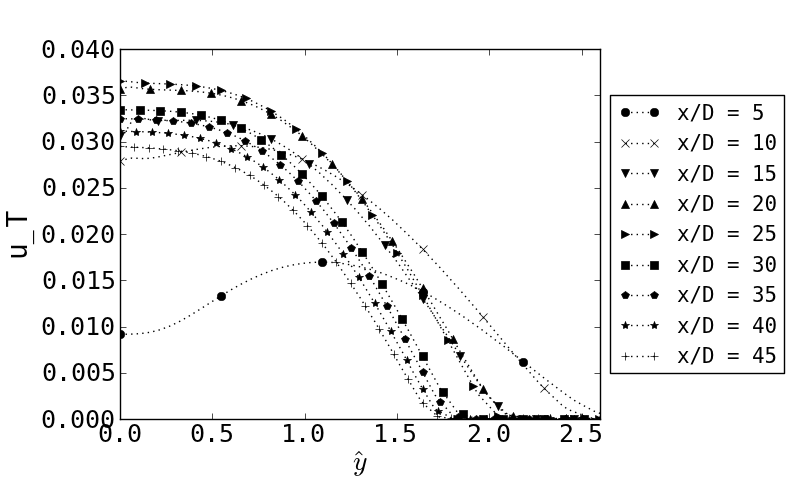
\includegraphics[width=0.5\textwidth]{../thesis/figuras/chap5/selfsimilar/selfsimilar_nut.png}} &\\
\end{tabular}
 \caption{Numerical results showing the evolution to self-similar profiles of the following gas phase properties: (a) dimensionless mean axial velocity - $\hat{U}_x$, (b) dimensionless turbulent kinetic energy - $\hat{k}$ - and (c) dimensionless turbulent viscosity - $\hat{\nu}_t$. The different curves show the profiles for the correspondent axial coordinate indicated in the legend.}
\label{fig: selfsimilar_profile}
\end{figure}

\begin{figure}[!htb]
 \centering
\begin{tabular}{cc}
 \subfloat[]{\label{fig: ssS}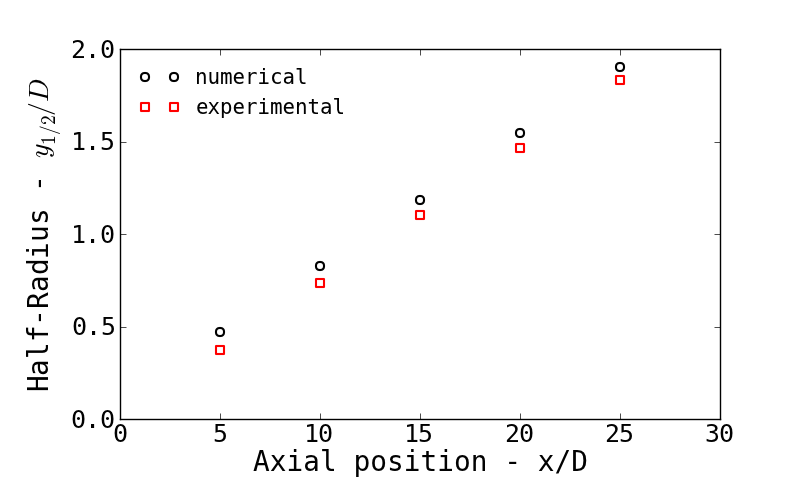
\includegraphics[width=0.5\textwidth]{../thesis/figuras/chap5/selfsimilar/selfsimilar_spread.png}} & \subfloat[]{\label{fig: ssP}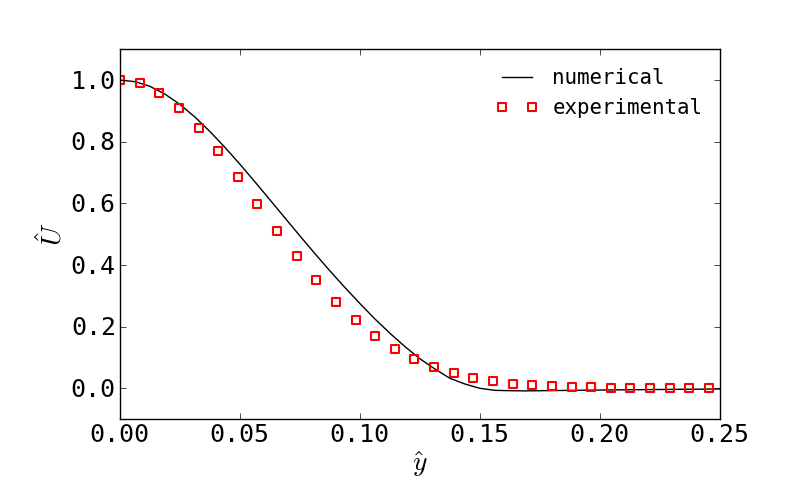
\includegraphics[width=0.5\textwidth]{../thesis/figuras/chap5/selfsimilar/selfsimilar_num_exp.png}}
\end{tabular}
 \caption{(a) Half-radius as a function of the axial coordinate in the experiment and in the simulation.  (b) Self-similar radial profile of the numerical and the experimental dimensionless axial velocity - $\hat{U}_x$. The measurements were obtained from \citet{chen}.}
\label{fig: selfsimilar_spread}
\end{figure}


\begin{figure}[!htb]
 \centering
\begin{tabular}{cc}
 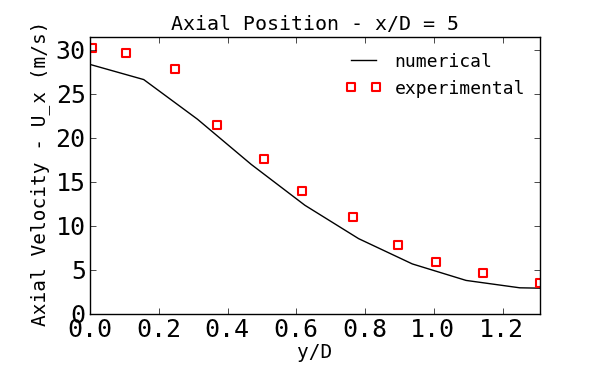
\includegraphics[width=0.5\textwidth]{../thesis/figuras/chap5/Ux/Ux_gas/Ux_gas5.png} & 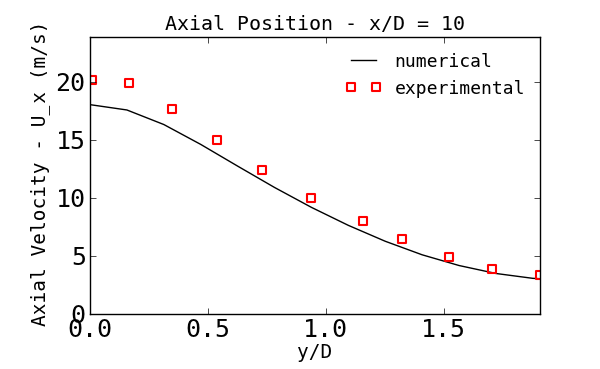
\includegraphics[width=0.5\textwidth]{../thesis/figuras/chap5/Ux/Ux_gas/Ux_gas10.png} \\
(a) & (b) \\
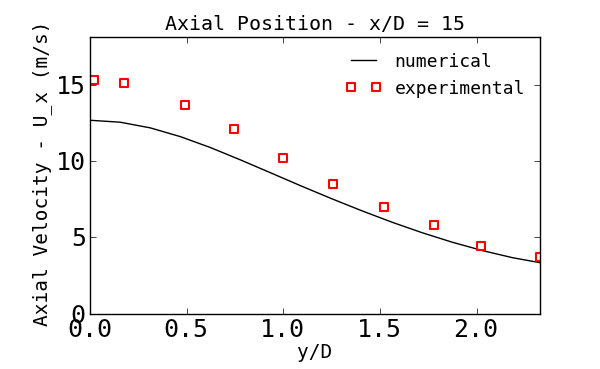
\includegraphics[width=0.5\textwidth]{../thesis/figuras/chap5/Ux/Ux_gas/Ux_gas15.png} & 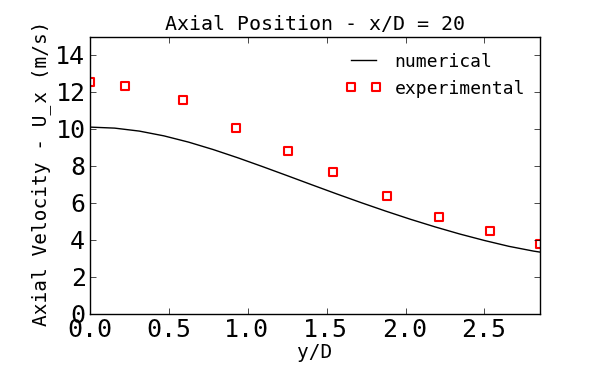
\includegraphics[width=0.5\textwidth]{../thesis/figuras/chap5/Ux/Ux_gas/Ux_gas20.png} \\
(c) & (d) \\
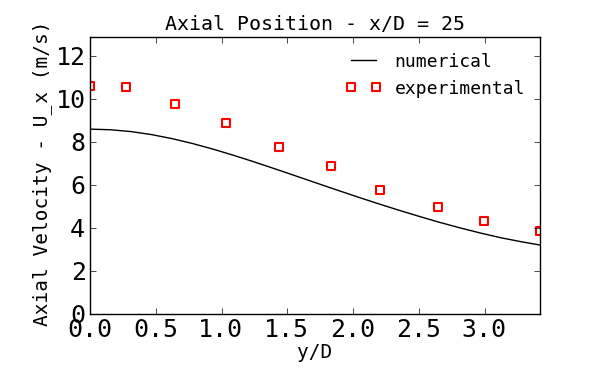
\includegraphics[width=0.5\textwidth]{../thesis/figuras/chap5/Ux/Ux_gas/Ux_gas25.png} &   \\
(e) & \\
\end{tabular}
 \caption{Measured and computed radial profiles of the mean axial velocity of the gas phase ($\tilde{U}_x$). The measurements were obtained from \citet{chen}.}
 \label{fig: Ux_gas}
\end{figure}


\begin{figure}[!htb]
 \centering
\begin{tabular}{cc}
 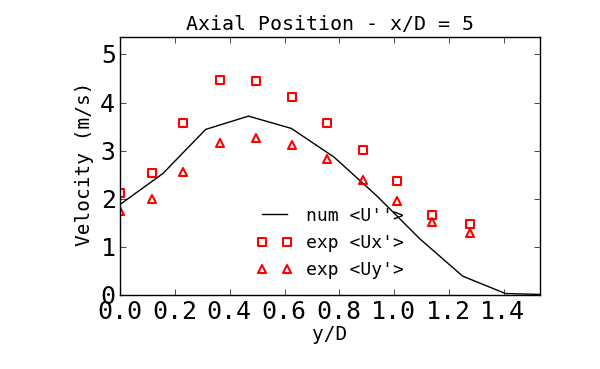
\includegraphics[width=0.5\textwidth]{../thesis/figuras/chap5/UU/UUx5.png} & 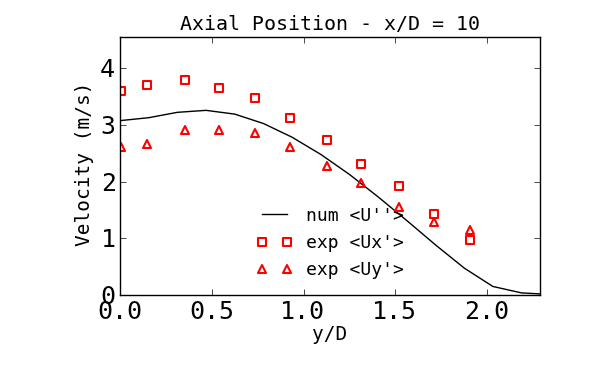
\includegraphics[width=0.5\textwidth]{../thesis/figuras/chap5/UU/UUx10.png} \\
(a) & (b) \\
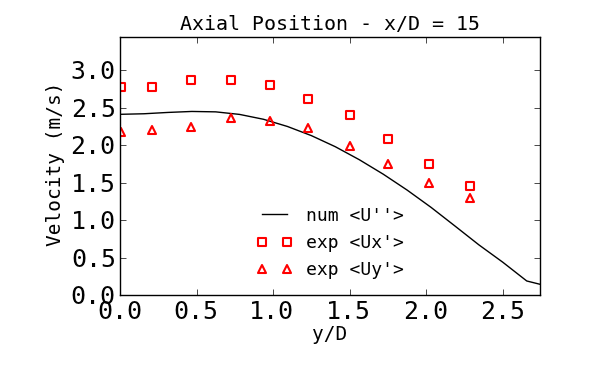
\includegraphics[width=0.5\textwidth]{../thesis/figuras/chap5/UU/UUx15.png} & 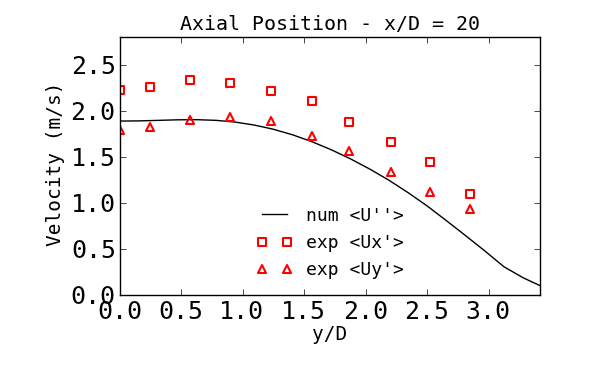
\includegraphics[width=0.5\textwidth]{../thesis/figuras/chap5/UU/UUx20.png} \\
(c) & (d) \\
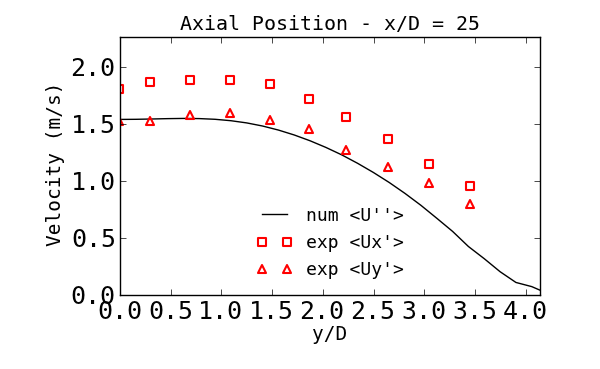
\includegraphics[width=0.5\textwidth]{../thesis/figuras/chap5/UU/UUx25.png} &  \\
(e) & \\
\end{tabular}
 \caption{Measured radial profiles of the gas phase velocities $<U''_x>$ and $<U''_y>$ and the characteristic velocity defined for the k-epsilon model $<U''>=\sqrt{2/3 k}$ obtained from the simulation. The measurements were obtained from \citet{chen}.}
\label{fig: UUx}
\end{figure}


\begin{figure}[!htb]
 \centering
\begin{tabular}{cc}
 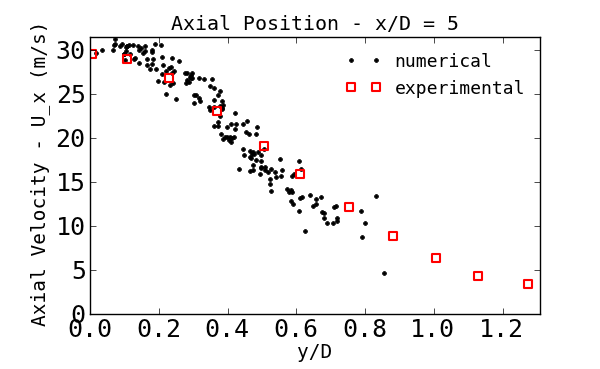
\includegraphics[width=0.5\textwidth]{../thesis/figuras/chap5/Ux/Ux_drops/Ux_x5.png} & 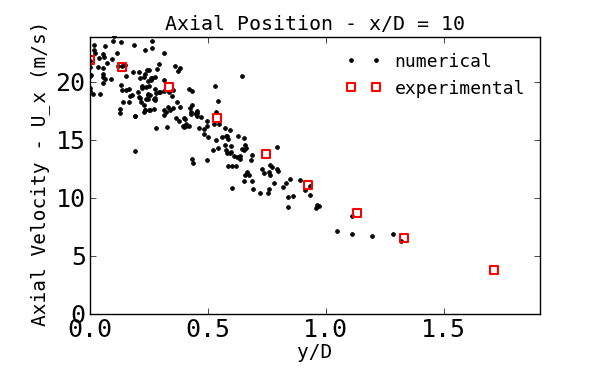
\includegraphics[width=0.5\textwidth]{../thesis/figuras/chap5/Ux/Ux_drops/Ux_x10.png} \\
(a) & (b) \\
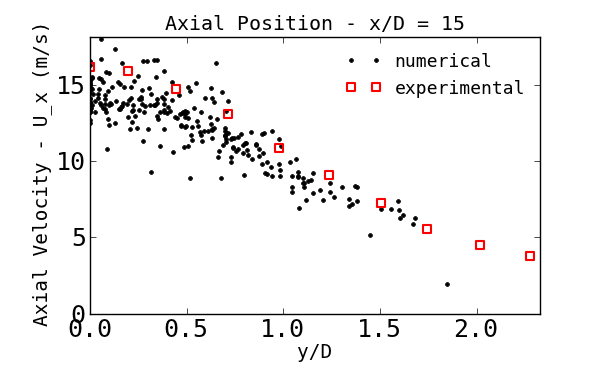
\includegraphics[width=0.5\textwidth]{../thesis/figuras/chap5/Ux/Ux_drops/Ux_x15.png} & 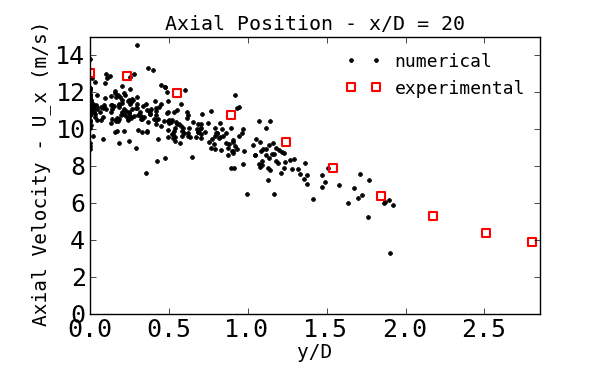
\includegraphics[width=0.5\textwidth]{../thesis/figuras/chap5/Ux/Ux_drops/Ux_x20.png} \\
(c) & (d) \\
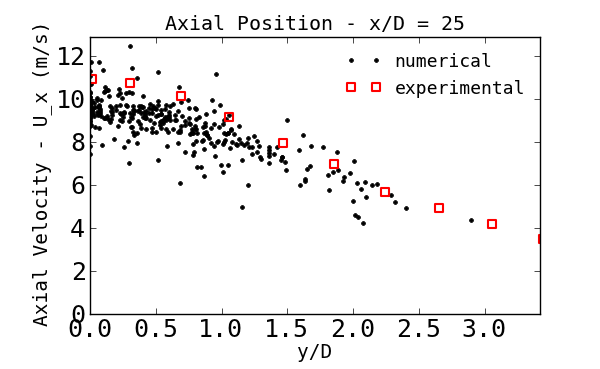
\includegraphics[width=0.5\textwidth]{../thesis/figuras/chap5/Ux/Ux_drops/Ux_x25.png} &   \\
(e) & \\
\end{tabular}
 \caption{Red squares are the measured radial profile of the mean axial velocity of droplets ($\tilde{U}_{d,x}$) in the size class of $10\mu m <D<20\mu m$. Scattered black dots are the computed velocities for each droplet in the numerical simulation. The measurements were obtained from \citet{chen}.}
 \label{fig: Ux}
\end{figure}


\begin{figure}[!htb]
\centering
  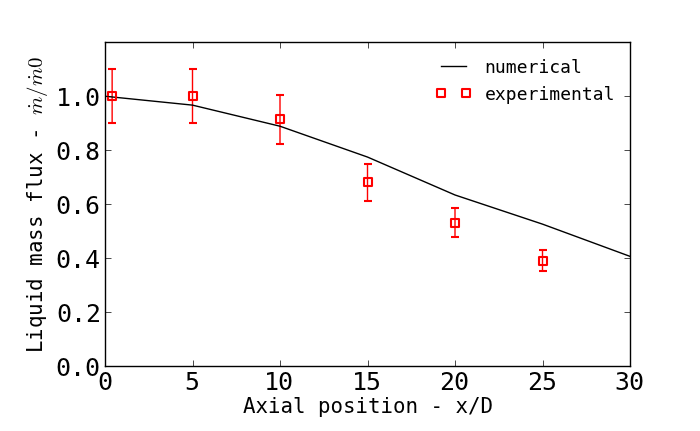
\includegraphics[width=0.6\textwidth]{../thesis/figuras/chap5/massflow/drop_mflux.png}
\caption{Droplet mass flow rate at four axial locations. The measurements were obtained from \citet{chen}.}
\label{fig: droplet_flux}
\end{figure} 


\begin{figure}[!htb]
 \centering
\begin{tabular}{cc}
 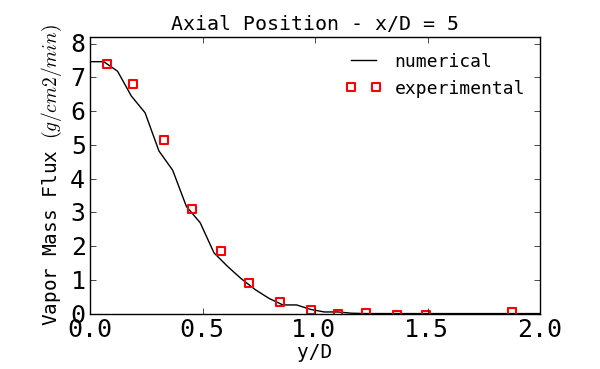
\includegraphics[width=0.45\textwidth]{../thesis/figuras/chap5/massflow/mvapor5.png} & 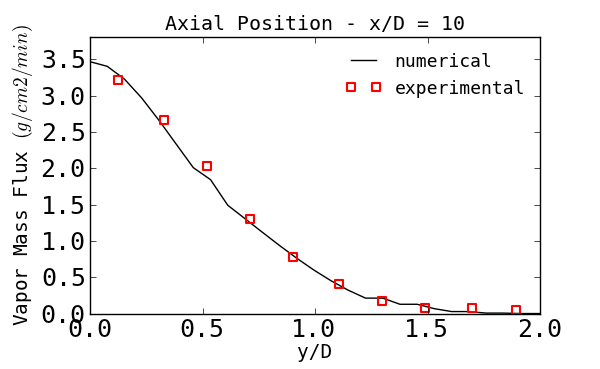
\includegraphics[width=0.45\textwidth]{../thesis/figuras/chap5/massflow/mvapor10.png} \\
(a) & (b) \\
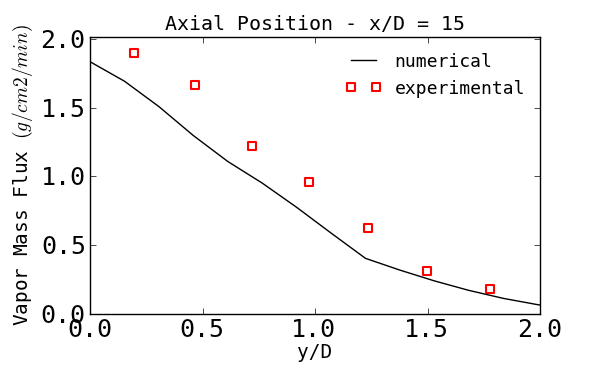
\includegraphics[width=0.45\textwidth]{../thesis/figuras/chap5/massflow/mvapor15.png} & 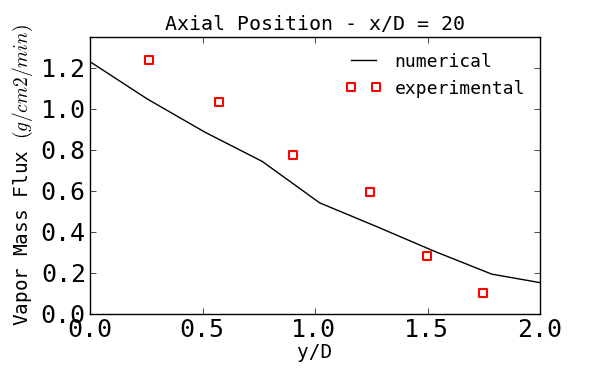
\includegraphics[width=0.45\textwidth]{../thesis/figuras/chap5/massflow/mvapor20.png} \\
(c) & (d)
\end{tabular}
 \caption{Radial profiles of mean axial mass flux of acetone vapor: $\dot{m}''_{ac}=\rho \bar{Y}_{ac} \tilde{U}_x$. The measurements were obtained from \citet{chen}.}
 \label{fig: vapor_flux}
\end{figure}


\begin{figure}[!htb]
 \centering
\begin{tabular}{c}
 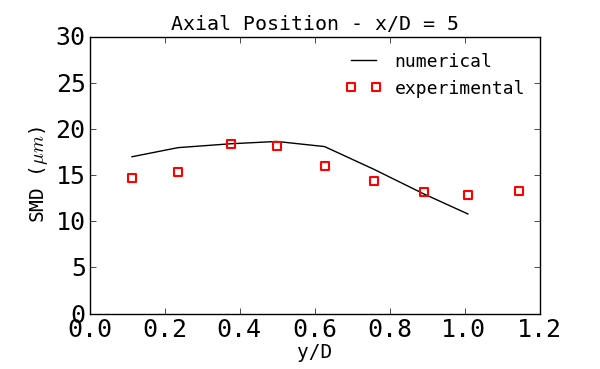
\includegraphics[width=0.5\textwidth]{../thesis/figuras/chap5/smd/smd5.png} \\
(a) \\
 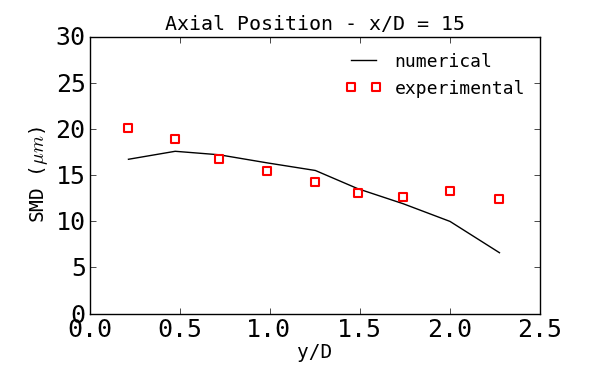
\includegraphics[width=0.5\textwidth]{../thesis/figuras/chap5/smd/smd15.png} \\
(b) \\
 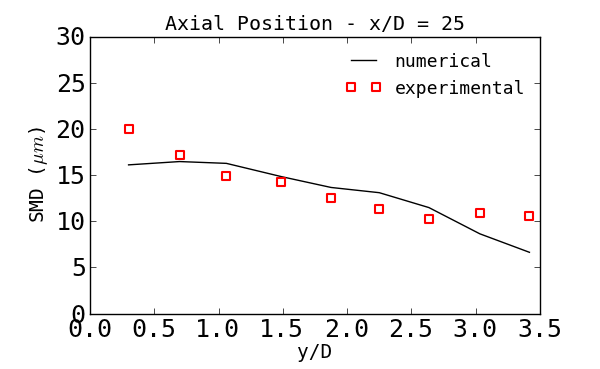
\includegraphics[width=0.5\textwidth]{../thesis/figuras/chap5/smd/smd25.png} \\
(c) 
\end{tabular}
 \caption{Numerical and experimental radial profiles of Sauter mean diameter (SMD). The measurements were obtained from \citet{chen}.}
 \label{fig: SMDprofile}
\end{figure}

\end{document}

%%
%% End of file `elsarticle-template-1a-num.tex'.
